\documentclass[12pt]{article}
 
\usepackage[margin=1in]{geometry} 
\usepackage{amsmath,amsthm,amssymb}
\usepackage{hyperref}
\usepackage{graphicx}
\usepackage{xcolor}
\usepackage[many]{tcolorbox}
\tcbuselibrary{listings}
\usepackage{listings}
%jari:
\usepackage{enumitem}

\definecolor{lg}{HTML}{f0f0f0}

\newtcblisting{pycode}{
    colback=lg,
    boxrule=0pt,
    arc=0pt,
    outer arc=0pt,
    top=0pt,
    bottom=0pt,
    colframe=white,
    listing only,
    left=15.5pt,
    enhanced,
    listing options={
        basicstyle=\small\ttfamily,
        keywordstyle=\color{blue},
        language=Python,
        showstringspaces=false,
        tabsize=2,
        numbers=left,
        breaklines=true
    },
    overlay={
        \fill[gray!30]
        ([xshift=-3pt]frame.south west)
        rectangle
        ([xshift=11.5pt]frame.north west);
    }
}

\lstset{
    language=Python,
    basicstyle=\small\ttfamily,
}

 
\begin{document}
 
\title{Exercise 4}
\author{Jari Mattila - 35260T\\
ELEC-E8125 - Reinforcement Learning}

\maketitle

\section*{Task 1}

The training performance plots are presented below for Task 1a using 
handcrafted feature vector $\phi(s) = [s,|s|]^T$ in Figure~\ref*{fig:fig1} and Task 1b 
using radial basis function representations in Figure~\ref*{fig:fig2}.
\newline

\begin{figure}[h] 
	\centering  % Remember to centre the figure
    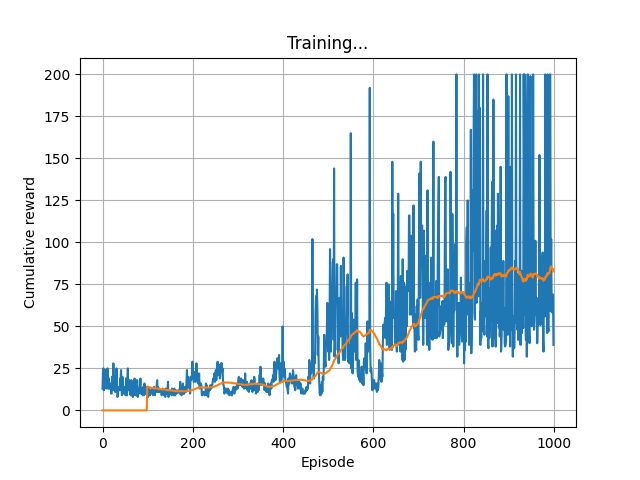
\includegraphics[width=0.9\columnwidth]{img/Figure_1_task_1a_cumulative_reward.png}
	\caption{Training performance using handcrafted feature vector $\phi(s) = [s,|s|]^T$.}
	\label{fig:fig1}
\end{figure}

\begin{figure}[h] 
	\centering  % Remember to centre the figure
    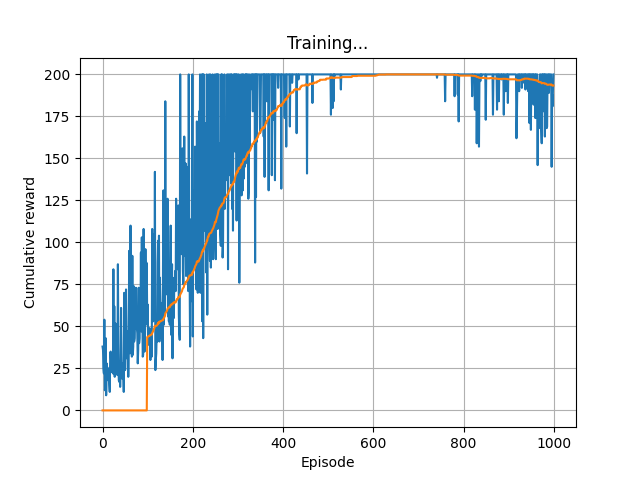
\includegraphics[width=0.9\columnwidth]{img/Figure_2_task_1b_cumulative_reward.png}
	\caption{Training performance using radial basis function representations.}
	\label{fig:fig2}
\end{figure}

\noindent
Source files: main\_task1.py, rbf\_agent\_task1a.py, rbf\_agent\_task1b.py 


\section*{Question 1}

Would it be possible to learn accurately Q-values for the Cartpole
problem using linear features (by passing the state directly to a linear regressor)? Why/why
not?
\newline

Learning Q-values for the Cartpole problem accurately using linear features can be difficult because the linear model cannot model dependencies between the features.
For example, in the Cartpole problem the high angular velocity can be either good or bad depending on the angle - this cannot be taken into account by the linear model (for details see Section 9.5 of Sutton's book).

\pagebreak


\section*{Task 2}

The implementation of Task1 has been modified to perform minibatch updates and
use experience replay in the following. The training performance plots are presented below for Task 2a using handcrafted feature vector $\phi(s) = [s,|s|]^T$ in Figure~\ref*{fig:fig3} and Task 2b using radial basis function representations in Figure~\ref*{fig:fig4}.

\begin{figure}[h] 
	\centering  % Remember to centre the figure
    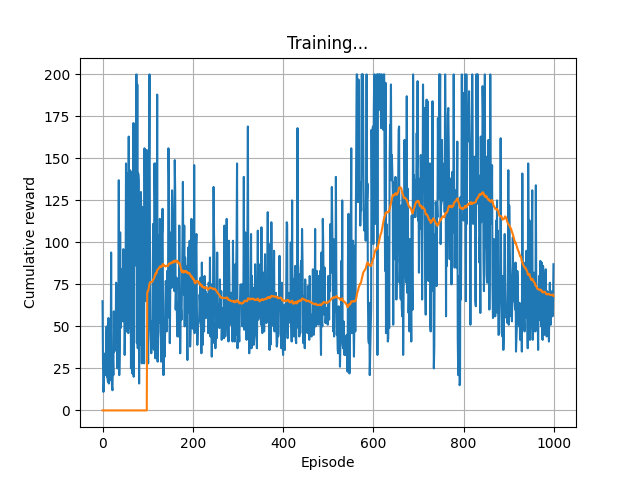
\includegraphics[width=0.9\columnwidth]{img/Figure_3_task_2a_cumulative_reward.png}
	\caption{Training performance using handcrafted feature vector $\phi(s) = [s,|s|]^T$.}
	\label{fig:fig3}
\end{figure}

\begin{figure}[h] 
	\centering  % Remember to centre the figure
    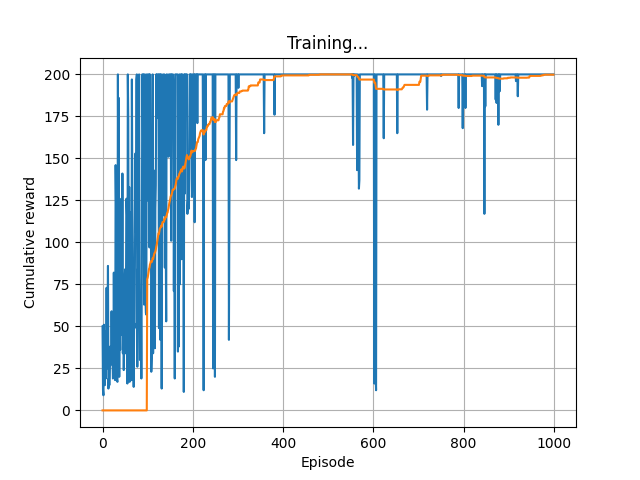
\includegraphics[width=0.9\columnwidth]{img/Figure_4_task_2b_cumulative_reward.png}
	\caption{Training performance using radial basis function representations.}
	\label{fig:fig4}
\end{figure}

\noindent
Source files: main\_task2.py, rbf\_agent\_task2a.py, rbf\_agent\_task2b.py 


\section*{Question 2}

Figure 2 (from ex4.pdf) shows the training performance of all four methods from Task 1, together
with grid-based learning from Exercise 3 evaluated using GLIE with a = 50.

\section*{Question 2.1}

How does the experience replay affect the learning performance?
\newline 

The experience replay clearly accelerates convergence to the optimum training performance in all cases presented in Figure 2. This is also quite understandable because the experience replay uses up to 32 times more data for training in the considered CartPole case. 


\section*{Question 2.2}

Discuss the benefits and cons of using hand-crafted features. As an example, you can refer to 
the given hand-crafted feature and more complex features like
$\phi(s) = [s_x, s_{\dot{x}}, \operatorname{cos}(s_{\theta}), \operatorname{sin}(s_{\theta}), s_{\dot{\theta}}]^T$.
\newline

The RBF kernel representation of non-linear features comprises 230 features that is clearly superior to the hand-crafted features of type $\phi(s) = [s, abs(s)]$ with 8 features. This simple feature model with 8 features may not take into account of the feature dependencies in the best possible way, which results in poorer performance.


\section*{Question 2.3}

Do grid based methods look sample-efficient compared to any of the
function approximation methods? Why/why not?
\newline

The grid based method are not very sample efficient compared to any of the
function approximation methods because, e.g. in the CartPole environment, they require thousands of episodes for convergence, which is achieved in hundreds of episodes with function approximation. 


\section*{Task 3}

The best action in terms of $x$ and $\theta$ for $\dot{x}=0$ and $\dot{\theta}=0$ learned with RBF with experience replay is presented below for Task 3 in Figure~\ref*{fig:fig5}.
The state-space was discretized for $x$ and $\theta$ using the default values of Ex. 3: $[x_{min}, x_{max}] = [-2.4, 2.4]$ and $[\theta_{min}, \theta_{max}] = [-0.3, 0.3]$.

\begin{figure}[h] 
	\centering  % Remember to centre the figure
    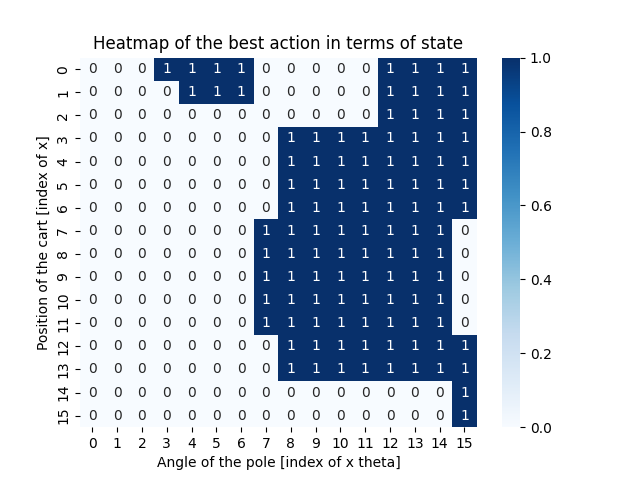
\includegraphics[width=0.9\columnwidth]{img/Figure_5_task_3_heatmap.png}
	\caption{Heatmap for the best action in terms of $x$ and $\theta$.}
	\label{fig:fig5}
\end{figure}


\noindent
Source files: main\_task3.py 



\section*{Task 4}

Training performance using DQN implementation in CartPole environment
is presented below for Task 4 in Figure~\ref*{fig:fig6}. 
\newline

\begin{figure}[h] 
	\centering  % Remember to centre the figure
    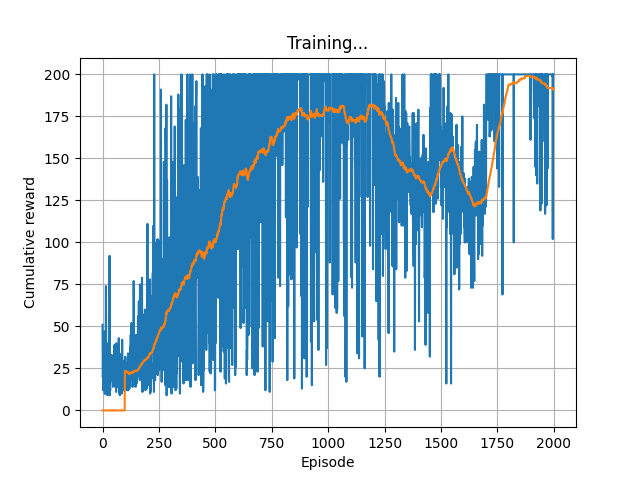
\includegraphics[width=0.9\columnwidth]{img/Figure_6_task_4a_cumulative_reward.png}
	\caption{Training performance using DQN implementation in CartPole environment.}
	\label{fig:fig6}
\end{figure}


The results of the LunarLander environment were unfortunately not ready for the report.
\newline

\noindent
Source files: main\_task4.py, dqn\_agent\_task4.py 


\section*{Question 3.1}

Can Q-learning be used directly in environments with continuous action spaces?
\newline

Q-learning can be applied to both discrete and continuous spaces.
The obvious approach is to discretize state space, and for particularly large state spaces, some form of functional approximation (such as via a neural network) can be used for the action value.


\section*{Question 3.2}

Which steps of the algorithm would be difficult to compute in case of
a continuous action space? If any, what could be done to solve them?
\newline

Evaluating the maximum in the Q learning equation can become problematic and less accurate for large continuous action spaces. One solution might be to use some actor-critic algorithms.


\pagebreak



\bibliographystyle{ieeetr}
\bibliography{template}  % Modify template with your bibliography name
\end{document}
